\section{Results} \label{results}
This sections presents results of the performance measurement experiments as described in Section \ref{methodology}. Because the experiments are specific to GTS, we start by commenting on the usability of the test environment and the deployment characteristics of the overlay solutions. Subsequently we present the results of the synthetic and the application benchmark respectively. 

\subsection{Usability GTS} \label{usabilitygts}
The GTS has proven to be an excellent environment for us to perform our measurements in. The extensive documentation and rapid support enabled us to deploy topologies, specifically catered to our experiments. Still, some shortcomings in the service regarding the usability and functionality have been identified throughout the course of the project. Shortcoming we experienced are:

\begin{itemize}
  \setlength\itemsep{-1pt}
  \item Unstable VPN initialization to the topology;
  \item VMs which fail to finish booting on multiple occasions;
  \item VMs permanently losing connectivity with the provisioning network (\texttt{eth0});
  \item Not all DSL-features appear to be fully functional;
  \item Limited control over VM resources, physical placement and imaging;
  \item Limited control over virtual NIC of the VMs.
\end{itemize}
Mostly, these shortcomings were caused due to general availability issues. However, they did not highly impact our ability to perform the research. More significant were the limited control options in the DSL and limited control over the networking interface of the virtual machine as they limited the amount of overlay solutions we were able to evaluate, as discussed in Section \ref{methodology}.

Whilst performing the experiments we noticed that the virtual machines deployed in GTS are relatively limited in terms of performance. By default each VM is assigned a single-core vCPU with a default speed of 2 gigahertz (GHz). Problems occurred when running performance measurements with \texttt{iperf}. The vCPU is unable to generate enough network traffic to saturate the 1 Gbps link connected to the virtual machines. Performance-wise, the only attribute which can be altered regarding the VM via the DSL is the speed of the processor with the \texttt{cpuSpeed} attribute. However, even when scaling up the \texttt{cpuSpeed} attribute to an arbitrarily high number, the speed of the processor is capped at 2.5GHz by OpenStack. Moreover, when attempting to deploy a full mesh with an increased \texttt{cpuSpeed}, the instance fails to deploy. Increasing the amount of cores per vCPU is not a documented attribute and as such does not seem to be a publicly available API call.

A trivial solution would be to limit the speed of the network interface card (NIC) via \texttt{ethtool}. However, attempting to change the speed of the interface within the virtual machine results in an error and is not supported by the VM. Another option was to limit the speed of the ports attached to the containers. For this purpose the \texttt{lineRate} attribute can be specified in the DSL whilst defining the ports. However, the \texttt{lineRate} attribute is set at 1 Gbps by default and only accepts increments of 1 Gbps. Lastly, the speed of the link between the containers can be defined within the DSL by specifying the \texttt{capacity} attribute. The GTS user guide notes that the default value is 10 Mbps which doesn't seem to be valid \cite{userguide}. Additionally, when statically defining the \texttt{capacity} to be 100 Mbps, the limitation does not seem to get applied. Arbitrary \texttt{iperf} measurements between containers still indicate speeds far north of the limit. Therefore we resorted to setting a software limit on the interface by using Wonder Shaper in the star topology experiment. This is also explained in Section \ref{startopo}

Fortunately the GTS is being frequently updated which means that some of the identified shortcomings may be fixed in newer iterations of the service. Additionally, some of the shortcomings may be caused due to the fact that we are limited to the 2.0 DSL while the service is currently running on v3.0.1. An updated user guide might solve of the issues related to deployment and control of resources. 

\subsection{Overlay evaluation}
As previously discussed in Section \ref{methodology}, only Calico was infeasible to deploy due to the limited control over the VM NIC in GTS. Flannel, Weave and the native overlay driver were fairly straight forward to set up. During the deployment we have noticed that Weave is by far the easiest overlay to deploy due to the fact that Weave uses CRDT to share the network state between Weave nodes. The other overlay solutions all require a separate key-value store for this purpose, effectively making the overall configuration more complex. In our experiments this was achieved by by deploying a single-key value store in one of the sites. However, in a real world deployment where process resilience is an important factor, a clustered key-value store distributed over multiple nodes may be desirable. This inherently means that an overlay network with these solutions requires management of another separate distributed system. Due to Weave's ease of deployment the solution seems to be especially suited for Agile development and rapid prototyping.

In operation we have noticed that the control method of the overlay varies between each solution. For example, Calico and Weave deploy separate containers which run the main overlay processes for routing and state exchange. Flannel on the other hand creates a service, running on each host machine. In the case of \texttt{libnetwork} the overlay is controlled by the already in place Docker engine. Although we are impartial to the method for controlling the overlay we do note that in an environment with limited resources, the overlay process or container(s) may contend for the CPU. As discussed in Section \ref{usabilitygts}, whilst performing our synthetic benchmark, the CPU utilization is 100\%. Nevertheless, no significant performance deterioration was measured between the native overlay driver and the evaluated overlay solutions. The full results of this experiment are presented in Section \ref{synthetic}.


\subsection{Base infrastructure performance}
As we were unable to control the placement of the virtual machines on a specific host within the topology instances, we initially verify that the node placement within a site is of no consequence to the performance. Figure \ref{fig:ALL_AMS_LJU_MEANLAT} presents a point-to-point measurement between virtual machines in the Amsterdam and Ljubljana sites. The measurements show an almost identical mean latency regardless of the underlying host the VMs are placed on. Additionally, the results in Appendix \ref{app:Baseline} show that currently no day/night cycle exists within GTS. 

\begin{figure}[H]
   \centering
   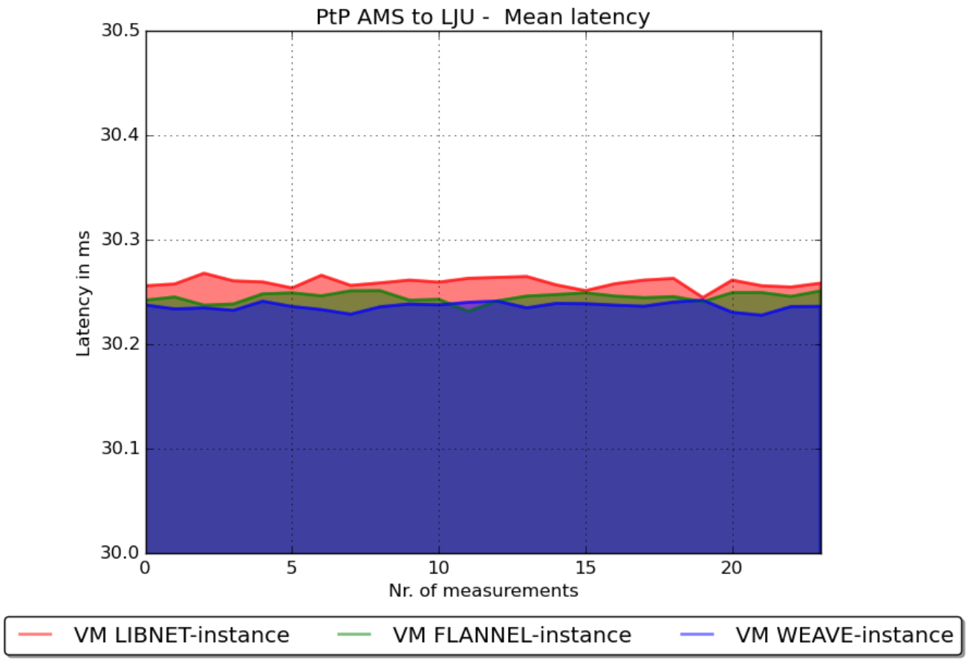
\includegraphics[scale=0.6]{img/ALL_AMS_LJU_MEANLAT.png}
   \caption{Single site VM measurements within three instances }
   \label{fig:ALL_AMS_LJU_MEANLAT}
\end{figure}

This means that later on, we can safely compare the overlay performances on the VMs which reside on different topology instances and possibly on different physical hosts. Based on the measurements above we can assume that all physical hosts within a site are identical in resources and utilization. Additionally, the absence of a day-night cycle and the insignificant amount of jitter indicates that there is little to no concurrent use of GTS taking place.

\subsection{Overlay performance} \label{synthetic}
Subsequently, we evaluate the general degradation of performance when introducing the overlay solutions into the equation. We started with the point-to-point measurements in the full mesh topology using \texttt{netperf}. In doing so, we have seen no significant differences in the jitter between the VMs and docker containers in any of the overlays. Any discrepancy within these results are small enough ($<$ 0.1 ms) to contribute to the fact that tests were ran subsequently to one another. When comparing overlay performances between each other, similar results are seen as portrayed in Table \ref{tab:PtP_Overlays_Latency}. Some outliers exist due to the limited amount of measurements that could be taken.
\\
\begin{table}[!ht]
\centering
\begin{tabular}{@{}lllll@{}}
\toprule
\textbf{Circuit} & \textbf{Instance} & \multicolumn{3}{c}{\textbf{In Milliseconds (ms)}} \\
\textbf{} & \textbf{} & \textit{\textbf{Min. Latency}} & \textit{\textbf{Mean Latency}} & \textit{\textbf{99th \% Latency}} \\ \midrule
AMS – MIL & Libnet & 36.3 & 36.5 & 37.0 \\
 & Weave & 36.2 & 36.5 & 37.0 \\
 & Flannel & 42.5 & 42.9 & 43.0 \\ \midrule
AMS – LJU & Libnet & 30.1 & 30.3 & 31.0 \\
 & Weave & 29.8 & 30.3 & 31 \\
 & Flannel & 29.8 & 30.3 & 31.0 \\ \midrule
AMS – BRA & Libnet & 17.6 & 17.7 & 18.0 \\
 & Weave & 17.4 & 17.7 & 18.0 \\
 & Flannel & 17.4 & 17.7 & 18.0 \\ \midrule
MIL – LJU & Libnet & 61.8 & 62.1 & 62.4 \\
\textit{} & Weave & 59.8 & 59.8 & 60.0 \\
\textit{} & Flannel & 55.6 & 55.8 & 56.0 \\ \midrule
\textit{MIL – BRA} & Libnet & 12.7 & 13.0 & 14.0 \\
\textit{} & Weave & 12.9 & 13.1 & 14.0 \\
\textit{} & Flannel & 12.9 & 13.1 & 14.0 \\ \midrule
\textit{BRA – LJU} & Libnet & 47.1 & 47.4 & 48.0 \\
\textit{} & Weave & 43.1 & 59.5 & 130.0 \\
\textit{} & Flannel & 43.1 & 43.3 & 44.0 \\ \bottomrule
\end{tabular}
\caption{Point-to-point latency measurements through the overlays }
\label{tab:PtP_Overlays_Latency}
\end{table}

Next, we saturate the link using \texttt{iperf}. Strangely enough, as figure \ref{fig:sub1} illustrates, we found that the TCP throughput in most cases resulted in the container out-performing the VM it is running on. The UDP throughput displayed in figure \ref{fig:sub2} shows a very different pattern. 

\begin{figure}[H]
\centering
\begin{subfigure}{.5\textwidth}
  \centering
  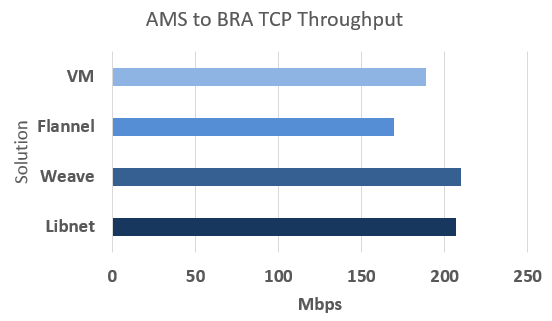
\includegraphics[scale=0.5]{img/PtP_All_TCP.PNG}
  \caption{TCP throughput}
  \label{fig:sub1}
\end{subfigure}%
\begin{subfigure}{.5\textwidth}
  \centering
  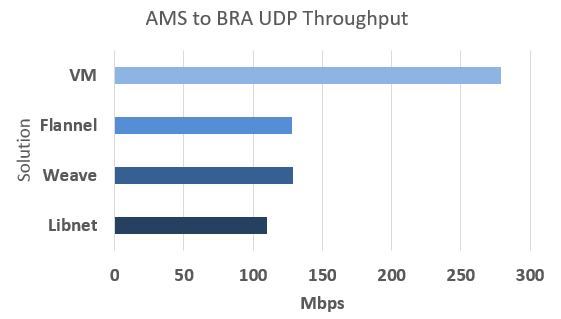
\includegraphics[scale=0.5]{img/PtP_All_UDP.PNG}
  \caption{UDP throughput}
  \label{fig:sub2}
\end{subfigure}
\caption{UDP and TCP throughput as measured on the Amsterdam - Bratislava circuit}
\label{fig:UDP_TCP_MSMT}
\end{figure}

The measured data indicates that the overlay solutions do not perform well during UDP testing. The full results of the experiment are presented in Appendix \ref{app:PtP}. Figure \ref{fig:UDP_TCP_MSMT} presents the results of the Amsterdam - Bratislava circuit. However, the measured anomalies are not specific to an individual circuit as is shown in Appendix \ref{app:PtP_through}. In some measurements the overlay outperforms the underlay whereas in other scenarios the opposite is true. 

Regarding the UDP throughput, Claassen examined similar behavior and hypothesized that the anomaly may be caused due to \texttt{iperf} consuming more CPU cycles for measuring the jitter of the UDP packets \cite{jorisclaassen2015}. However, in his work no anomalies were found regarding TCP throughput. This observation will be further explored in the discussion in Section \ref{discussion}. 

\subsection{Media streaming scenario}
After the point-to-point measurements, the performance of the overlays in a star-topology was evaluated by stressing a central node with a gradually increasing amount of concurrent sessions. In this scenario performance is defined by measuring the jitter on the link and the bit rate of the stream as measured on the client side. The streaming media measurements have been performed sequentially and within a single topology instance. 

Figure \ref{fig:sub3} presents the jitter results from the streaming test with a varying amount of Faban workers for the underlay and each of the overlays, specifically on the Bratislava - Amsterdam circuit. Little to no jitter is measured with a low amount of workers (e.g. one and three workers) is used as there is no real congestion on the link. In both cases the jitter remains below or around 0.5 milliseconds.  However, when the total amount of requested streams is increased to nine, artificial congestion is created on the 10 Mbps rate limited link. This inherently causes the jitter to increase. 

\begin{figure}[!ht]
\centering
\begin{subfigure}{.5\textwidth}
  \centering
  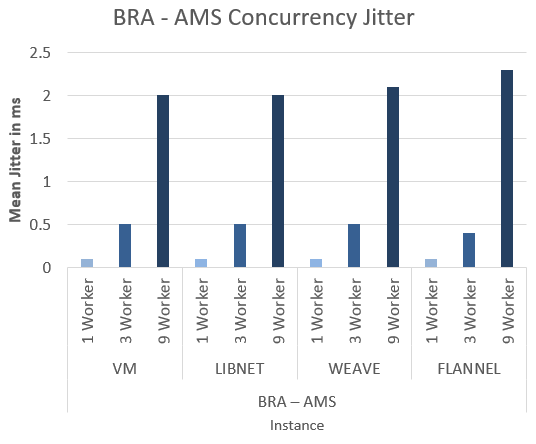
\includegraphics[scale=0.5]{img/All_Streaming_jitter.PNG}
  \caption{Jitter measurements}
  \label{fig:sub3}
\end{subfigure}%
\begin{subfigure}{.5\textwidth}
  \centering
  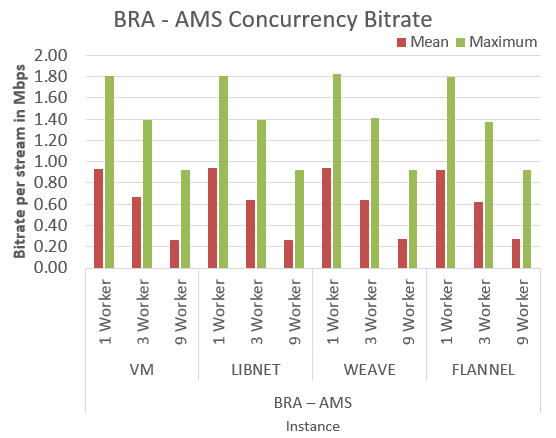
\includegraphics[scale=0.5]{img/All_Streaming_TP.PNG}
  \caption{Bit rate measurements}
  \label{fig:sub4}
\end{subfigure}
\caption{Concurrency measurements through the overlays and VM in the star topology}
\label{fig:PtP_All_TCP.PNG}
\end{figure}

During the stresstest the amount of jitter fluctuates between approximately 2 and 2.3 milliseconds. Figure \ref{fig:sub3} shows a slight increase in jitter for Weave and Flannel respectively, but this fluctuation is not significant and may be flattened out over the course of additional consecutive measurements. Furthermore, the difference in jitter between the virtual machines and the overlay solutions are not significant.

The measured values are below the recommendations from Cisco which state that a video stream should have less than 30 milliseconds of one way jitter \cite{szigeti_hattingh_2004}. Still, Claypool and Tanner show that even low amounts of jitter can have a high impact on the perceived quality of a video stream by end users \cite{claypool1999effects}. Client- and server-side buffering can be utilized to cope with slight increases in jitter.

As expected, the results from the bit rate evaluation indicate that bit rates per stream deteriorate when the amount of requesting clients increase. Figure \ref{fig:sub4} illustrates that the deterioration holds a very similar pattern between the underlay and the overlay solutions. There is no significant performance difference between a specific overlay solution and the underlay. Appendix \ref{app:stream} presents the full results of the media streaming scenario for each of the circuits as displayed in figure \ref{fig:stream_topology}.

